\parx
Figure \ref{fig:cn_command_palette} shows the Command Palette which is a tool
for faster accessing and performing of commands through filtering all commands
available in the software. The Command Palette can be accessed by pressing the keyboard
shortcut of \textbf{ctrl + shift + p}.

\begin{figure}[H]
	\centering
	\captionsetup{justification=centering}
	\captionsetup[figure]{list=yes}
	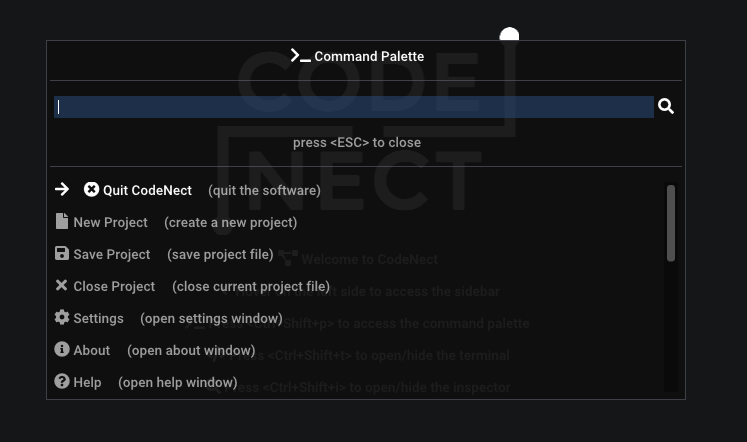
\includegraphics[width=\linewidth]{media/sc_command_palette.png}
	\caption[Command Palette in CodeNect]{Command Palette in CodeNect}
	\label{fig:cn_command_palette}
\end{figure}

